% \documentclass[handout, xcolor=table]{beamer}
\documentclass[xcolor=table]{beamer}

\usepackage{fixcmex} % fix binomials
\usepackage{xskak}

%-----------------------[ Macros ]----------------------------------------------%

%-----------------------[ Packages ]-------------------------------------------%

% \usepackage[utf8]{inputenc} % not needed for LuaLaTex
\usepackage[brazilian]{babel}
% \usepackage[english]{babel}
\usepackage[T1]{fontenc}
\usepackage{lmodern}
\usepackage{amsfonts}
\usepackage{indentfirst}
\usepackage{xspace}
\usepackage{setspace}
\usepackage{geometry}
\usepackage{mathtools}
\usepackage{amsmath}
\usepackage{amsthm}
\usepackage{subcaption}
\usepackage{pdfpages}
\usepackage{hanging}
\usepackage{pdfpages}
\usepackage{nicefrac}
\usepackage{graphicx}
\usepackage[labelformat=empty]{caption}
\usepackage[shortlabels]{enumitem}
\usepackage{booktabs, multirow} % for borders and merged ranges
% \usepackage[hyperpageref]{backref}
% \usepackage[
%   scr=boondox, % heavily sloped
%   cal=esstix % slightly sloped
% ]{mathalpha}
\usepackage{xmpmulti}
\usepackage{appendixnumberbeamer}
\usepackage{emoji}
% \usepackage{newpxtext} % other font

% Tikz:
\usepackage{tikz}
% \usetikzlibrary{ipe} % ipe compatibility library
\usetikzlibrary{calc, arrows, arrows.meta, patterns}

\usepackage{macrossty}

%-----------------------[ Colors ]---------------------------------------------%

\definecolor{red}{rgb}{1,0,0}
\definecolor{blue}{rgb}{0,0,1}
\definecolor{green}{rgb}{0,1,0}
\definecolor{yellow}{rgb}{1,1,0}
\definecolor{orange}{rgb}{1,0.647,0}
\definecolor{gold}{rgb}{1,0.843,0}
\definecolor{purple}{rgb}{0.627,0.125,0.941}
\definecolor{gray}{rgb}{0.745,0.745,0.745}
\definecolor{brown}{rgb}{0.647,0.165,0.165}
\definecolor{navy}{rgb}{0,0,0.502}
\definecolor{pink}{rgb}{1,0.753,0.796}
\definecolor{seagreen}{rgb}{0.18,0.545,0.341}
\definecolor{turquoise}{rgb}{0.251,0.878,0.816}
\definecolor{violet}{rgb}{0.933,0.51,0.933}
\definecolor{darkblue}{rgb}{0,0,0.545}
\definecolor{darkcyan}{rgb}{0,0.545,0.545}
\definecolor{darkgray}{rgb}{0.663,0.663,0.663}
\definecolor{darkgreen}{rgb}{0,0.392,0}
\definecolor{darkmagenta}{rgb}{0.545,0,0.545}
\definecolor{darkorange}{rgb}{1,0.549,0}
\definecolor{darkred}{rgb}{0.545,0,0}
\definecolor{lightblue}{rgb}{0.678,0.847,0.902}
\definecolor{lightcyan}{rgb}{0.878,1,1}
\definecolor{lightgray}{rgb}{0.827,0.827,0.827}
\definecolor{lightgreen}{rgb}{0.565,0.933,0.565}
\definecolor{lightyellow}{rgb}{1,1,0.878}
\definecolor{black}{rgb}{0,0,0}
\definecolor{white}{rgb}{1,1,1}

%-----------------------[ Commands ]-------------------------------------------%

\newcommand\mycomment[1]{} % block comment

\newcommand{\dist}{\text{dist}}
\newcommand{\cost}{\text{cost}}
\newcommand{\opt}{\text{OPT}}
\newcommand{\makespan}{\emph{makespan}}

\newcommand{\cala}{\mathcal{A}}
\newcommand{\calb}{\mathcal{B}}
\newcommand{\calg}{\mathcal{G}}
\newcommand{\cali}{\mathcal{I}}
\newcommand{\call}{\mathcal{L}}
\newcommand{\calo}{\mathcal{O}}
\newcommand{\cals}{\mathcal{S}}
\newcommand{\calt}{\mathcal{T}}

\newcommand{\N}{\rm I\!N}
\newcommand{\overeps}{\nicefrac{1}{\varepsilon}}
\newcommand{\B}{$\bullet$}

\newcommand\rest[2]{\left.{#1}\right|_{#2}} % function restriction

\newcommand\set[1]{\{#1\}}

\DeclarePairedDelimiter\ceil{\lceil}{\rceil}
\DeclarePairedDelimiter\floor{\lfloor}{\rfloor}
\DeclareMathOperator*{\argmax}{arg\,max}
\DeclareMathOperator*{\argmin}{arg\,min}

\newcommand{\XSAT}{\textrm{XSAT}} % Exact SAT
\newcommand{\rXSAT}{$(2,1)$-\XSAT} % Exact SAT with 2 positive, 1 negative occurences of each variable
\newcommand{\rXthreeSAT}{\mbox{$1$-in-$3$-SAT$_{(2,1)}$}}%{$(2,1)$-X3SAT} % Exact SAT with 2 positive, 1 negative occurences of each variable, and clauses with size <= 3
\newcommand{\kXSAT}{$k$-\textrm{True} \rXSAT}
\newcommand{\kXthreeSAT}{$k$-\textrm{True} \rXthreeSAT}

%-----------------------[ Proof Environments ]---------------------------------%

% \newtheorem{definition}{Definição}
\newtheorem{thm}{Teorema}
\newtheorem{cor}{Corolário}
\newtheorem{conj}{Conjectura}
\newtheorem{lema}{Lema}
\newtheorem{obs}{Observação}
\newtheorem{remark}{Remark}
\newtheorem{proposition}{Proposition}

\newcounter{finalframe}
\newcommand{\stopcounter}{
  \setcounter{finalframe}{\insertframenumber}
}

\newcommand{\resumecounter}{
  \setcounter{framenumber}{\value{finalframe}}
}

\newcommand{\inccounter}{
  \setcounter{framenumber}{\value{finalframe} + 1}
}

%-----------------------[ Template ]-------------------------------------------%

\mode<presentation> {
    \usetheme[sectionpage=none, progressbar=frametitle, block=fill]{moloch} % modern fork of the metropolis theme
    \setbeamertemplate{footline}[frame number] % to replace the footer line in all slides with a simple slide count
}
\setbeamerfont{footnote}{size=\tiny}
\setbeamertemplate{navigation symbols}{}
\setbeamertemplate{footnote}{%
    \hangpara{2em}{1}%
    \makebox[2em][l]{\tiny\insertfootnotemark}%
    \hspace{-1em}\tiny\insertfootnotetext\par\vspace{0.2cm}%
}
\setbeamercolor{background canvas}{bg=white}

% Enumerate setup:
\def\labelenumi{\textbf{\arabic{enumi}.}}

% Lists setup:
\beamerdefaultoverlayspecification{<+->}

%-----------------------[ (Sub)Section Slides ]--------------------------------%

\AtBeginSection[]{
    \begin{frame}
    \vfill
    \centering
    \setbeamercolor{title}{bg=mDarkTeal,fg=black!2}
    \begin{beamercolorbox}[sep=8pt,center,shadow=true]{title}
        \usebeamerfont{title}\insertsectionhead\par%
    \end{beamercolorbox}
    \vfill
    \end{frame}
}

% \makeatletter
% \newcommand{\subseqslide}{
% \begin{frame}
%   \setbeamercolor{title}{bg=mDarkTeal,fg=black!2}
%   \centering
%   \begin{minipage}{22em}
%     \raggedright
%     \begin{beamercolorbox}[sep=8pt,center,shadow=true]{title}
%         \usebeamerfont{title}\insertsectionhead\par%
%     \end{beamercolorbox}
%     \usebeamertemplate*{progress bar in section page}
%     \par
%     \ifx\insertsubsectionhead\@empty\else%
%       \vskip-.6\baselineskip
%       \usebeamercolor[fg]{subsection title}%
%       \usebeamerfont{subsection title}%
%       \insertsubsectionhead{}
%     \fi
%   \end{minipage}
%   \par
%   \vspace{\baselineskip}
% \end{frame}
% }

% \AtBeginSubsection[]{%
% \subseqslide

% \setcounter{tocdepth}{3}
% \frame<beamer>{ 
%   \frametitle{}
%   \centering
%   \begin{minipage}{20em}
%   \tableofcontents[
%     currentsection,currentsubsection,sectionstyle=show/hide,subsectionstyle=show/shaded/hide,subsubsectionstyle=show/show/hide/hide
%   ]    
%   \end{minipage}
% }
% }
% \makeatother

%-----------------------[ Title page ]-----------------------------------------%

\title{Algoritmos de Aproximação para Problemas NP-completos em Grafos Planares}

\titlegraphic{
  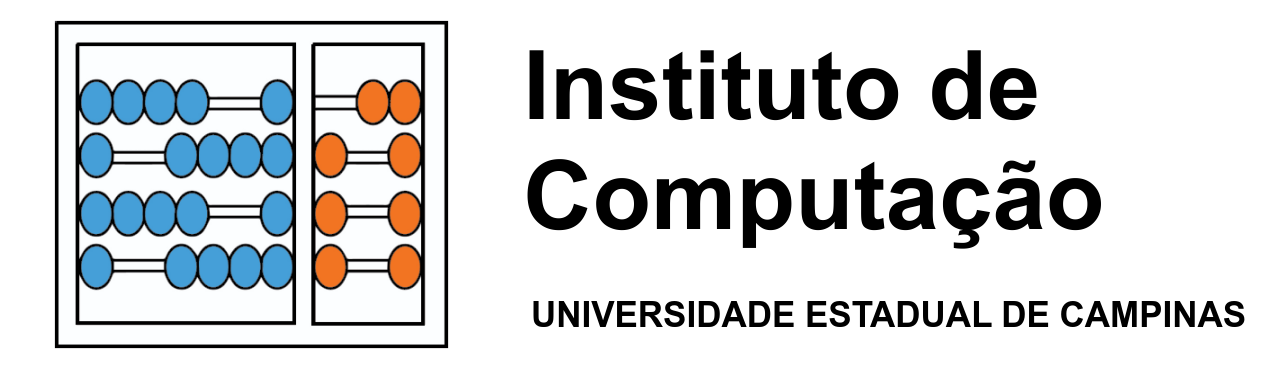
\includegraphics[height=1.cm]{logos/ic.png}
  \hfill
  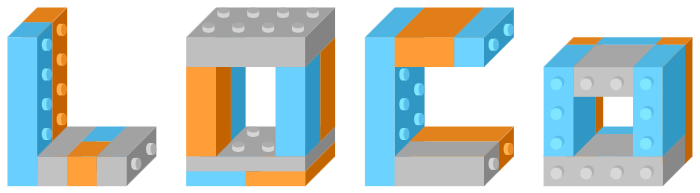
\includegraphics[height=0.85cm]{logos/loco.png}
}

\author{
Lucas de Oliveira Silva - 220715
}

% \institute{}

\date{\vfill\hfill 26 de Junho de 2025}

\begin{document}

\hyphenpenalty=10000

\begin{frame}[plain]
  \titlepage
\end{frame}

%------------------------------------------------------------------------------%

\section{Introdução}
\begin{frame}{Problema Exemplo}
    \defproblemaOPT
        {Conjunto Independente Máximo (CI)}
        {Grafo $G = (V, E)$.\pause}
        {$S \subseteq V$ tal que $|E(G[S])|=0$, com $|S|$ máximo.}
\end{frame}

\begin{frame}{Dificuldade}
    \begin{thm}[\cite{Ga79}]
        O problema do Conjunto Independente Máximo é NP-difícil, mesmo em grafos cúbicos e planares.
    \end{thm}
\end{frame}

\begin{frame}{Limitante de Aproximação}
    \begin{thm}[\cite{Hstad99}]
        Seja $n$ o número de vértices de um grafo, e $\varepsilon > 0$. \medskip \pause

        Não existe aproximação com fator $O(n^{\varepsilon - 1})$ para CI, a menos que $P = NP$.
    \end{thm}
\end{frame}

\begin{frame}{Algoritmo para Árvores}
    \begin{thm}[folclore]
        Seja $T$ uma árvore. É possível computar um conjunto independente máximo de $T$ em tempo polinomial.
    \end{thm}
\end{frame}


\section{Preliminares}
\begin{frame}{Grafos Outerplanares}
    \begin{minipage}{\linewidth}
        \centering
        
\includegraphics[height=5cm]{images/outerplanar.png}
    \end{minipage}
\end{frame}

\begin{frame}{Grafos $k$-outerplanares}
    \centering
    \Large Exemplo para $k=3$:
    \bigbreak
    \begin{minipage}{\linewidth}
        \centering
        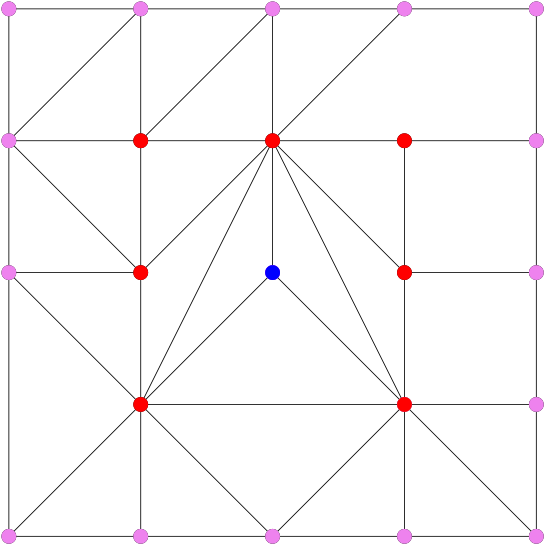
\includegraphics[height=6cm]{images/k-outer.png}
    \end{minipage}
\end{frame}

\begin{frame}{CI em Grafos $k$-outerplanares}
    \begin{lema}[1] \label{lema1}
        Existe um algoritmo por PD que resolve CI em grafos $k$-outerplanares em tempo $2^{O(k)} \cdot n$.
    \end{lema}
\end{frame}

\begin{frame}{Esboço da Prova}
    \begin{proof}
        \begin{lema}[\cite{Bod98}]
            Grafos $k$-outerplanares têm largura arbórea no máximo $3k - 1$.
        \end{lema}
        \bigbreak
        \begin{lema}[\cite{Cygan15}]
            Seja $G$ um grafo com $n$ vértices e largura arbórea $\leq k$. Então, CI em $G$ pode ser resolvido em tempo $2^k \cdot k^{O(1)} \cdot n$.
        \end{lema}
        \alt<3>{\qedhere}{\phantom\qedhere}
    \end{proof}
\end{frame}


\section{Resultado Principal}
\begin{frame}{Teorema Principal}
    \begin{thm}[1 \cite{Baker83}] \label{teo1}
            Existe um PTAS para CI em grafos planares, com tempo $O(2^{O(\nicefrac{1}{\varepsilon})} \cdot n)$.
        \end{thm}
\end{frame}

\begin{frame}{Observação}
    \centering
    \vspace{1cm}
    \pause
    \Large Assim como ogros, grafos planares têm camadas!
    \begin{minipage}{\linewidth}
        \centering
        \vspace{1.73cm}
        
\includegraphics[height=5cm]{images/shrek.png}
    \end{minipage}
\end{frame}

\begin{frame}{Exemplo}
    \begin{minipage}{\linewidth}
        \centering
        \only<1>{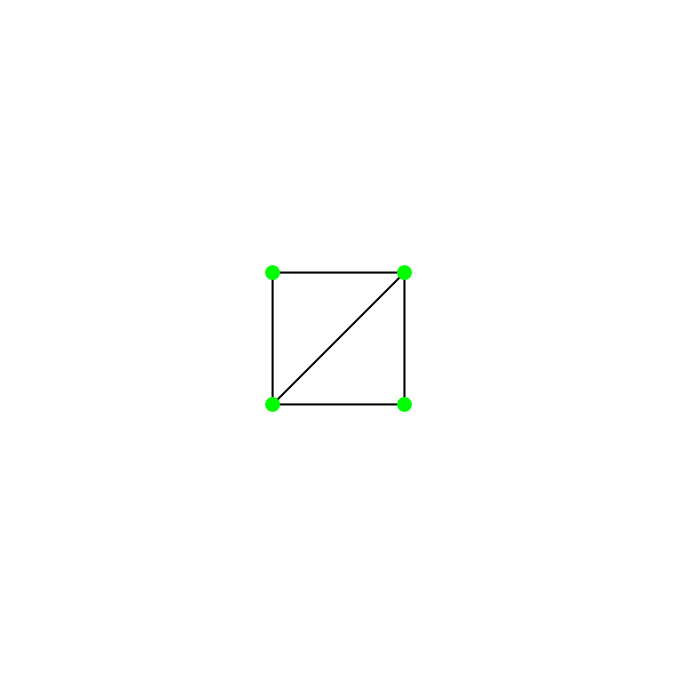
\includegraphics[height=6cm]{images/outer1.png}}
        \only<2>{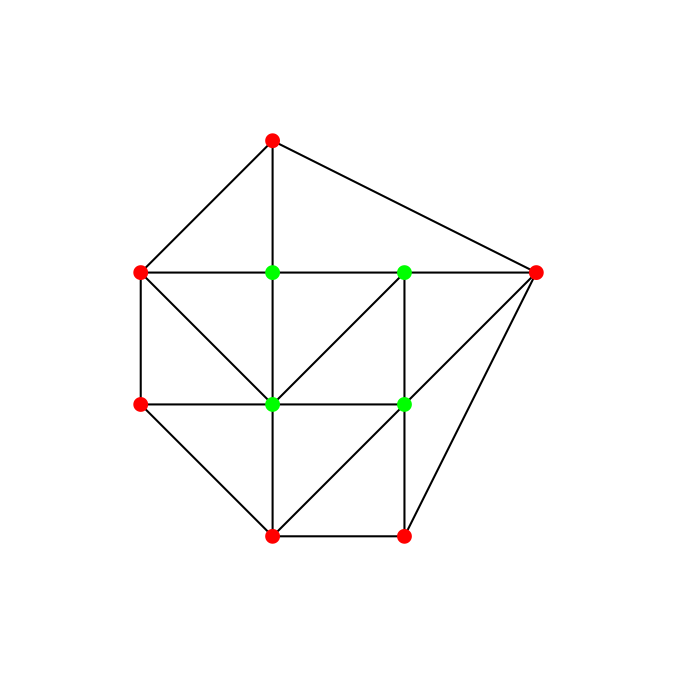
\includegraphics[height=6cm]{images/outer2.png}}
        \only<3>{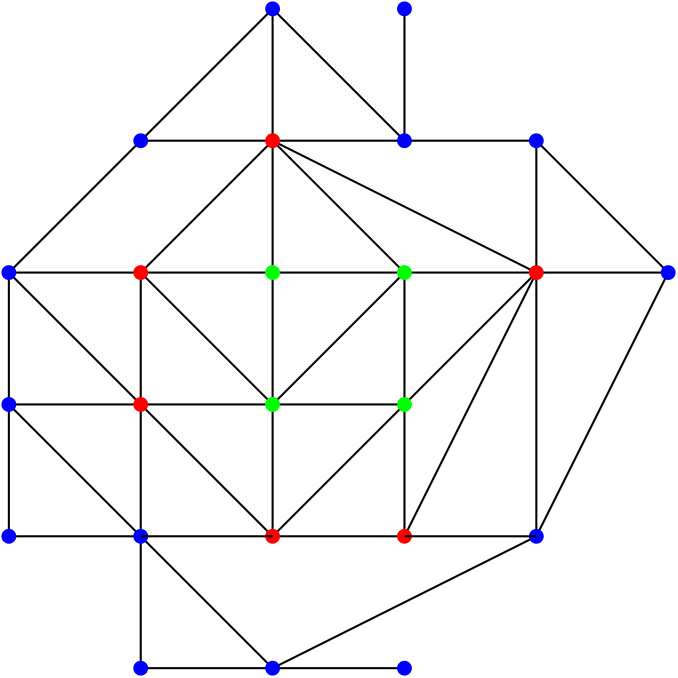
\includegraphics[height=6cm]{images/outer3.png}}
    \end{minipage}
\end{frame}

\begin{frame}{Preparação}
    Dado $G=(V, E)$ planar e $\varepsilon > 0$, definimos:
    \pause
    \begin{enumerate}[-]
        \item $k=\ceil{\nicefrac{1}{\varepsilon}}$;
        \item Para $0 \le i < k$, seja $S_i = \{L_j \mid j \equiv i \pmod k\}$
        \begin{enumerate}[-]
            \item Ex.: $k = 4 \Rightarrow S_1 = L_1 \cup L_5 \cup L_9 \cup \dots$
        \end{enumerate}
        \item $G_i = G[V - S_i]$.
    \end{enumerate}
\end{frame}

\begin{frame}{Decomposição em \emoji{onion}}
    \centering
    \Large $k=3$:
    \bigbreak
    \begin{minipage}{\linewidth}
        \centering
        \only<1>{
\includegraphics[height=5cm]{images/onion1.png}}
        \only<2>{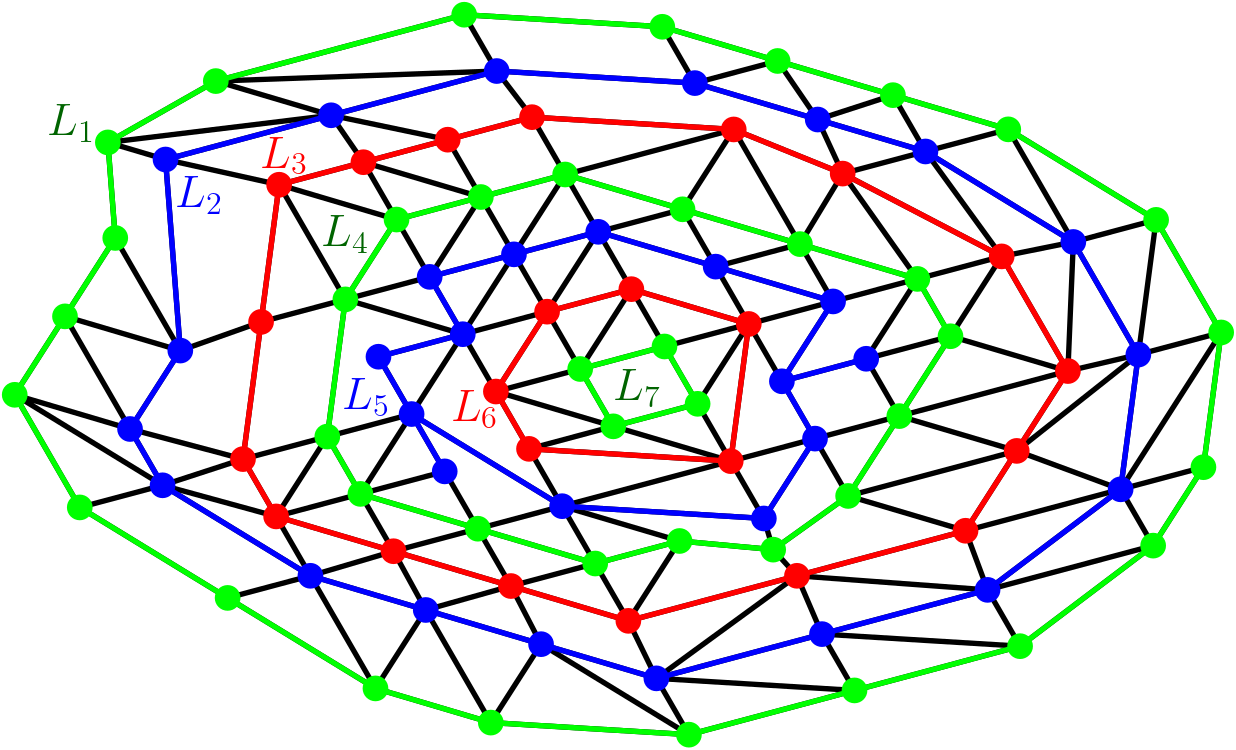
\includegraphics[height=5cm]{images/onion2.png}}
        \only<3>{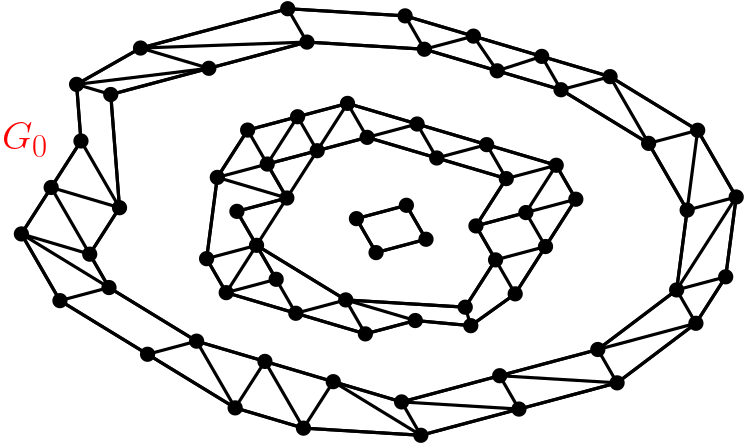
\includegraphics[height=5cm]{images/onion3.png}}
        \only<4>{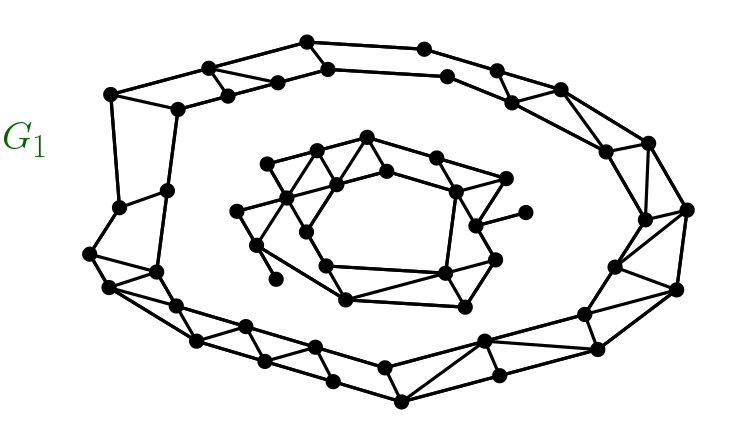
\includegraphics[height=5cm]{images/onion4.png}}
        \only<5>{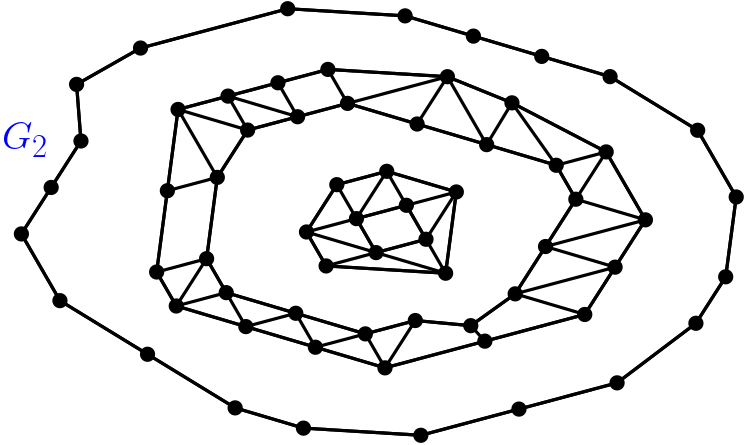
\includegraphics[height=5cm]{images/onion5.png}}
    \end{minipage}
\end{frame}

\begin{frame}{Solucionando $G_i$}
    \centering\Large
    Aplicamos o Lema \ref{lema1} em cada componente.
\end{frame}

\begin{frame}{Solução Ótima para $G_i$}
    \centering\Large
    Para cada $i$, geramos uma solução ótima $X_i$ de $G_i$.
    \bigbreak
    O tempo total gasto é $2^{O(k)} \cdot n = 2^{O(\nicefrac{1}{\varepsilon})} \cdot n$.
\end{frame}

\begin{frame}{Aproximação para $G$}
    \centering\Large
    Basta retornar o $X_\alpha$ de maior cardinalidade!
\end{frame}

\begin{frame}{Fator de Aproximação}
    \pause
    \setbeamercovered{transparent} % fade-in/fade-out lists
    \begin{proof}
        \begin{enumerate}
            \setlength\itemsep{1em}
            \item<2,8> Seja $O \subseteq V$ uma solução ótima;
            \item<3,8> $S_0, \dots, S_{k-1}$ particionam $V$;
            \item<4,8> Algum $i$ satisfaz $|O \cap S_i| \leq \nicefrac{|O|}{k}$;
            \item<5,8> $O \setminus S_i$ é independente em $G_i$;
            \item<6,8> Então $|X_\alpha| \ge |O \setminus S_i| = |O| - |O \cap S_i|$;
            \item<7,8> Portanto, $|X_\alpha| \ge \left(1 - \frac{1}{k}\right)|O| \ge (1 - \varepsilon) \cdot OPT$.
        \end{enumerate}
        \alt<8>{\qedhere}{\phantom\qedhere}
    \end{proof}
\end{frame}


\section{Conclusão}
\begin{frame}{Outros Resultados}
    \begin{thm}[\cite{Baker83}]
        Existe um PTAS para os seguintes problemas em grafos planares:

        \begin{enumerate}[]
            \item Conjunto Independente Máximo;
            \item \emph{Maximum Tile Salvage};
            \item Partição em Triângulos;
            \item $H$-Emparelhamento Máximo;
            \item Cobertura por Vértices Mínima;
            \item Conjunto Dominante Mínimo;
            \item Conjunto Dominante de Arestas Mínimo.
        \end{enumerate}
    \end{thm}
\end{frame}

\begin{frame}{Limitações}
    \centering
    A técnica de \emph{Shifting}/Baker é eficaz para problemas ``locais''~\dots
    \bigbreak\pause
    \dots~mas falha em casos como TSP ou Árvore de Steiner.
\end{frame}

\begin{frame}{Generalização}
    \centering\large
    \emph{Decomposição por contração} em grafos livres de $H$~\cite{Dem11}.
\end{frame}

\begin{frame}{Aplicação}
    \begin{thm}[\cite{Dem11}]
        Existe um PTAS para o TSP em grafos ponderados livres de $H$.
    \end{thm}
\end{frame}

\begin{frame}
  \large{\centerline{Obrigado a todos pela atenção...}}
  \Huge{\centerline{Fim.}}
\end{frame}

%-----------------------[ Bibliography ]---------------------------------------%

\appendix

\beamerdefaultoverlayspecification{}
\setbeamertemplate{bibliography item}[text]
\begin{frame}
  \frametitle{Bibliografia}
  {
    \tiny
    \bibliographystyle{alpha}
    \bibliography{bibliography}
  }
\end{frame}

%-----------------------[ Backup ]---------------------------------------------%


\end{document}
